%/\chapter{Fusão de evidências na detecção de bordas em Imagens PolSAR}
\chapter{Introdução}
\label{cap_acf}

\section{Aspectos gerais}

Neste trabalho estudaremos as imagens de radar de abertura sintética (\textit{Synthetic Aperture Radar} -- SAR) e as imagens de radar polarimétrico de abertura sintética (\textit{Polarimetric Synthetic Aperturadar} -- PolSAR).
Ambas requerem modelos e algoritmos adequados para o tratamento das suas características especiais.
Em particular, trabalharemos com técnicas de detecção de bordas.

No estudo de imagens PolSAR podemos citar diferentes técnicas, por exemplo, no trabalho de \citet{slf_2008} é usado modelagem eletromagnética para propor uma abordagem de detecção de bordas nas simulações de imagens PolSAR. 
%%% ACF Frase confusa:
Nos trabalhos de \citet{tlb, obw, flmc, fyf} podemos encontrar técnicas de detecção de bordas baseadas em métodos que estimam ouni gradiente, que funcionam usando uma janela deslizante, destacando através do cálculo do gradiente as bordas das imagens. 
Em \citet{obw} foi proposto o método de máxima verossimilhança para detectar a presença de bordas, em uma janela pré-definida de pixeis com a tarefa de encontrar bordas acuradas. 
O estudo de detecção de bordas, usando propriedades físicas das áreas estudadas, pode ser encontrado no trabalho de \citet{bf}, as quais utilizam cadeias de Markov. 
Em \citep{gfn} é descrita a comparação entre vários detectores de bordas que seguem a ideia deste trabalho. 
Técnicas baseadas nas modelagens estatísticas têm sido usadas na detecção de bordas em imagens SAR, podemos citar os trabalhos de \citet{gmbf, fbgm, horrit, gfn}. 
%%% ACF A revisão da literatura precisa ser mais informativa. São mencionadas abordagens completamente diferentes, sem que o leitor saiba as suas diferentes hipóteses de partida, nem os seus resultados. Essa parte é central para dar valor ao trabalho de doutorado.

Atualmente as pesquisas em \textit{Deep Learning} são muito importantes na área de sensoriamento remoto, aplicações são encontradas nas referências \citep{bac, ztmxzxf, tabmm, xstz}. 
As técnicas de \textit{Deep Learning} são usadas para segmentar ou classificar imagens, podendo auxiliar no processo de detecção de bordas. 

A área de fusão de imagens também é explorada neste trabalho. 
Um recente e interessante artigo, cujo autores são \citet{sglmla}, usa ideias do método \textit{random forest} aplicado em fusão de imagens PolSAR, adicionalmente, o artigo de \citet{sg} mostra outras técnicas de fusão de informação.  

O presente trabalho seguirá a abordagem de modelagem estatística, principalmente as técnicas descritas em \citep{fbgm, nhfc} usando a distribuição Wishart. Para realizar a fusão de informações temos como base as referências \citep{mit, sglmla, sg}. 

O objetivo deste trabalho é detectar bordas em cada polarização (canal) de uma imagem PolSAR e realizar a fusão das evidências de bordas, com a tarefa de melhorar a acurácia em relação a borda detectada, em cada polarização. A sequência de procedimentos pode ser descrita por:
\begin{itemize}%%% ACF Use o pacote "listing" para configurar e automatizar listas; com isso, poderá fazer referência a elas.
	\item[(i)] em cada polarização;
	\item[(ii)] especificar manualmente ou automaticamente a região de interesse (\textbf{ROI});
	\item[(iii)] em cada (\textbf{ROI}) calcular o centro de massa e a partir desse ponto traçar retas na direção radial de forma que garanta a existência de uma borda em cada reta;
	\item[(iv)] para todas as retas devemos analisar a variação das amostras, usando o método da máxima verossimilhança com o intuito de descobrir uma evidência de borda ou ponto de transição;
	\item[(v)] obtendo as evidências de bordas em todas as reta impostas, e repetindo o método em cada polarização, é realizado a média aritmética ou ponderada das evidências de bordas, para obter a fusão das mesmas;
	%%% ACF Aqui você se compromete com uma única técnica de fusão. É pouco para uma tese de doutorado.
	\item[(vi)] realizado a fusão das evidências de borda, teremos uma nuvem de pontos onde podemos aplicar métodos de regressão, usando para isso, o método dos quadrados mínimos para obter os resultados numéricos do presente trabalho.
\end{itemize}

Os itens (i) até (iv) tratam da detecção de borda que foram propostos nas seguintes referências bibliográficas \citep{gmbf, gmbf_sc, fbgm}, esses artigos usam a distribuição $G^{0}$ proposta por \citet{fmcs}. Neste trabalho usaremos a distribuição Wishart como na referência \citep{nhfc}. 

No item (v) a principal referência usada para fusão de evidências foi \citet{mit}, no item (vi) para o método dos quadrados mínimos foi usado a referência \citep{demmel}.

No presente trabalho o procedimento acima foi testado em imagens simuladas ou \textit{Phantons}. O resultado comparativo em relação as detecções de bordas nas polarizações nos mostrou uma estratégia de detecção de borda mais acurada. Os resultados alcançados devem ser testados em imagens PolSAR reais para verificar o desempenho e acurácia. 
\section{ Formação das imagens SAR}
O radar de abertura sintética (SAR) é o desenvolvimento tecnológico do radar de abertura real (RAR), o qual, de maneira geral trabalha com sensores ativos que transmitem micro-ondas e depois registram os ecos recebidos. Os radares usam plataformas tanto móveis como satélites, balões, veículos aéreos tripulados ou não quanto fixas, por exemplo, radares em aeroportos. Esses radares viajam em uma rota conhecida, transmitindo micro-ondas em direção ao alvo e recebendo micro-ondas ou ecos depois da interação com o alvo. 

Podemos afirmar que os radares têm fontes próprias de energia, ou seja, as micro-ondas são emitidas no próprio radar, por esse motivo são definidos como radares ativos, e adicionalmente, se possuirem uma antena para transmitir e receber os impulsos, são denominadas mono-estáticos. Importantes informações sobre radares podem ser encontradas na referência \citep{lp}, seus desenvolvimentos são norteados pelos princípios definidos a seguir:
\begin{itemize}
\item[(i)] possibilidade de uma antena transmitir um certo impulso eletromagnético (micro-ondas) em uma direção precisa; 
\item[(ii)] possibilidade de detectar com grande precisão o eco, depois da interação com o alvo, é atenuando com um processo que podemos chamar de espalhamento, onde a onda encontra o material do alvo induzindo uma corrente que gera uma energia eletromagnética irradiada em todas as direções, a maior parte dessa energia irradiada distancia-se do radar causando o espalhamento, não sendo possível detectar;
\item[(iii)] capacidade de medir o tempo entre a transmissão  e a recepção do impulso eletromagnético e, consequentemente, a distância entre o alvo e a antena;
\item[(iv)] habilidade de detectar vários alvos em grandes áreas a serem varridas.
\end{itemize}

A onda eletromagnética pode variar em comprimento e amplitude, dependendo da construção dos sensores para o radar em operação, uma característica importante dessas ondas é a capacidade de penetração no material analisado, dependendo do comprimento de onda, por exemplo, quanto maior o comprimento de onda, maior será a penetração no material analisado. 

Os radares podem produz imagens bidimensionais (2D) com resoluções distintas, dependendo do tipo de radar e da tecnologia empregada. As dimensões das imagens dependem respectivamente da resoluções nas direções de azimute e distância (\textit{range}). A direção de azimute é a mesma direção da rota do radar sendo perpendicular à direção da distância. A resolução na direção de azimute depende do comprimento $l$ da abertura antena de radar.  

Os radares que dependem diretamente dos comprimentos $l$ são os radares de abertura real (RAR), os quais têm uma grande restrição de uso em sensoriamento remoto, pois o comprimento da antena limita a resolução na direção de azimute, ou seja, para aumentar a resolução nesta direção, precisamos aumentar o comprimento da antena, o que pode ser inviável em satélites ou até mesmo em aviões, configurando-se em grande problema para essa área de pesquisa até os anos 50.  

Nos anos 50, pesquisadores fizeram avanços significativos para resolver a limitação tecnológica e desenvolveram uma técnica apta a sintetizar o efeito de uma antena muito longa, em uma antena de tamanho real. Para esse fim utilizaram o conhecimento na área de  processamentos de sinais em uma antena real para tornar possível a simulação de uma antena muito longa e, portanto, aumentar a resolução na direção do azimute. Essa descoberta é atribuída a Carl Wiley por volta de 1951.

O tipo de radar que utiliza a técnica, na qual uma antena real sintetiza uma antena longa, tornou-se conhecida como radar de abertura sintética (SAR), em 1954, Wiley registrou a patente do sistema SAR. O principal conceito físico para gerar a tecnologia dos sistema SAR, foi o efeito Doppler aplicados aos ecos dos radares. Devido ao avanço tecnológico no início da década de 50, um sistema SAR foi operacionalizado em torno de 1958. Consequentemente esse fato impulsionou fortemente a área de pesquisa relacionada com os sistemas SAR. 

Os dados provenientes do método de sintetização da antena real (SAR) são gravados de maneira única como uma faixa de posições para cada tempo avançado na direção da rota (azimute). No início do desenvolvimento dos sistemas SAR o armazenamento de dados foi um grande problema, para contorná-lo foi acoplado um sistema ótico nos radares para armazenar dados em filmes fotográficos. Atualmente devido ao desenvolvimento da eletrônica, o armazenamento de dados deixou de ser um problema nos sistemas SAR.

Nos sistemas SAR as ondas eletromagnéticas são representadas como imagens, que chamaremos de imagens SAR, geradas de forma que em cada ponto da direção azimute, o radar envia um impulso e recebe o sinal (eco), com o devido espalhamento. Esse sinal é armazenado ao longo da distância. Portanto, para cada tempo na direção do azimute geramos informações que serão armazenadas em uma linha de dados, tendo como resultado um mapeamento azimute \textit{versus} distância da energia recebida pelo radar, durante o tempo de aquisição de dados. Essas informações são típicas de armazenamentos em matrizes com as dimensões dependente da resolução inerente do radar.

Uma imagem SAR é visualizada em tons de cinza dependendo de como o alvo espalha a onda eletromagnética, sendo assim um alvo mais rugoso dá origem a pixeis mais claros, enquanto um alvo menos rugoso dá origem a pixeis mais escuros. 

Uma importante propriedade das imagens SAR é a transmissão e o recebimento de ondas eletromagnéticas em única direção, isto é, a onda pode ser transmitida e recebida tanto na direção horizontal como na vertical, configurando a polarização em uma das direções.

A generalização do processo SAR é conhecido como sistema polarimétrico SAR (PolSAR) definido como sendo a ciência de adquirir, processar e analisar o estado da polarização nas imagens de radar de abertura sintética, podemos dizer que é um sistema SAR capaz de medir mais de um estado de polarização. Em sistemas PolSAR as imagens de radares são formadas por ondas eletromagnéticas com várias combinações para as polarizações, tanto na transmissão como no recebimento das ondas, revelando uma melhor descrição do alvo em relação as imagens SAR. As imagens PolSAR têm o intuito de melhorar o entendimento do efeito do espalhamento de ondas pelos alvos levando, em conta as diferentes polarizações.

Os radares são usados de forma massiva desde os anos 40, principalmente para uso militar. Nos anos 50 houve a descoberta da tecnologia SAR, o que impulsionou um grande desenvolvimento na área levando a construção do primeiro radar de abertura sintética (SAR) comercial. O SEASAT foi o primeiro satélite orbital, operacional  e comercial projetado, seu lançamento foi em junho de 1978, a tabela (\ref{cap_acf_tab01}) mostra algumas características do SEASAT. 

\begin{table}[hbt]
	\centering
	\caption{Características do satélite SEASAT (SAR).}\label{cap_acf_tab01}
\begin{tabular}{@{}llr@{}} \toprule
	Características específicas& Valores operacionais  \\ \midrule
	Frequência           & \SI{1.275}{\GHz}  \\ 
	Altitude             & \SI{780}{\km}   \\
	Peso                 & \SI{2300}{\kilogram}   \\
	Ângulo de inclinação & \SI{\sim 23}{\degree}   \\
	Distância {\it range}& \SI{100}{\km}  \\
	Largura de banda     & \SI{19}{\MHz}   \\
	Banda - $L$          & \SI{23.5}{\cm} de comprimento de onda\\
	Polarização          & $HH$, onda emitida e recebida na direção horizontal \\
	Resolução            & $25 \times 25$  \\ \bottomrule

\end{tabular}
\end{table}
  
O projeto do SEASAT foi muito bem sucedido e estabeleceu definitivamente os sistemas SAR como área de pesquisa. Outros projetos de sistema SAR e PolSAR foram lançados e podem ser vistos na tabela (\ref{cap_acf_tab02}).

\begin{sidewaystable}
	\centering
	\caption{Características operacionais dos satélites SAR ou PolSAR.}\label{cap_acf_tab02}
\begin{tabular}{@{}llllllllr@{}} \toprule
Satélites      & 	SEASAT  &AIRSAR &SIR-C& Almaz&ERS-2& JERS-1& RADSAT-1&RADSAT-2 \\ \midrule
Nacionalidade       &EUA    &EUA&Alamanha-Itália&Rússia&Europa&Japão&Canadá&Canadá  \\ 
Lançamento          &1978   &1988        &1990  &1992  &1995 &1998  &1995  & 2003\\
C. de onda (\si{\cm}) (Banda) & 23.5 ($L$)&67 ($P$)/23.5 ($L$)/5.7 ($C$)&23.5 ($L$)/5.7 ($C$)/3.2 ($X$)&10 ($S$)&5.7 ($C$)&23.5 ($L$)&5.6 ($C$)&5.6 ($C$)\\
Polarização         &$HH$&$HH/HV/VV$&$HH/HV/VV$&$HH$&$VV$&$HH$&$HH$&$HH/HV/VV$\\
Ângulo de incidência&23&20-60&15-55&30-60&23&35&20-59&20-60\\
Distância (\si{\km})           &100&10-17&15-90&350&100&75&50-500&10-500\\
Resolução (\si{\m})         &25&2-8&10-60&10-30&30&18&10-100&3-100\\ \bottomrule
\end{tabular}
\end{sidewaystable}

Os símbolos $HH$, $HV$ e $VV$ representam as polarizações disponíveis nos radares, onde a primeira letra é a maneira como a onda é emitida e, a segunda letra é a maneira como a onda é recebida. Desta forma, quando aparece todas as combinações juntas temos um satélite com tecnologia PolSAR.

Os radares SAR e PolSAR possuem algumas características operacionais que podem ser resumidas nos seguintes itens:
\begin{itemize}
\item podem estar em plataformas elevadas, aeronaves tripuladas ou não, satélites orbitando a terra ou outros planetas;
\item é uma técnica de produção de imagem viável e prática;
\item possui alta resolução;
\item sintetiza longas aberturas de antenas;
\item os radares produzem imagens dia e noite;
\item o clima não interfere na captação de imagens;
\item os sistema de imagem SAR operam na região de micro-ondas do espectro eletromagnético, usualmente entre a banda $P-$ e a banda $K-$, a tabela (\ref{cap_acf_tab03}) mostra o espectro eletromagnético usado nas imagens SAR.
\end{itemize}
%%% ACF O texto está desordenado. As propriedades gerais do SAR/PolSAR deveriam estar antes das suas propriedades específicas
As aplicações das imagens SAR e PolSAR são intensas na área militar, porém existe um espectro de aplicações amplo, principalmente na iniciativa privada.  Devido a consolidação do satélite SEASAT podemos usar as imagens para o estudo de diversas áreas, como:
\begin{itemize}
\item sensoriamento remoto;
\item topografia;
\item oceanografia;
\item glaciologia;
\item agricultura;
\item geologia;
\item florestas;
\item alvos fixos ou em movimento;
\item monitoramento ambiental;
\item controle de derramamento de petróleo;
\item e no auxílio de sistemas óticos.
\end{itemize}
\begin{table}[hbt]
	\centering
	\caption{Espectro eletromagnético para a faixa de micro-ondas.}\label{cap_acf_tab03}
\begin{tabular}{@{}llc@{}} \toprule
	banda & Frequência $f$(\si{Ghz}) & Freq.$\times$C. de onda $\lambda(cm)$. \\\midrule
	$P$&$(<0.39, 0.39)$  & $0.3\times 100.0$  \\ 
	$L$&$(0.39-1.55)$  &  $1.0\times 30.0$\\ 
	$S$&$(1.55-3.90)$  &  $3.0\times 10.0$\\ 
	$C$&$(3.90-5.75)$  & $\sim(4.0\times 7.0)$ \\ 
	$X$&$(5.75-10.9)$  & $10.0\times 3.0$ \\ 
	$K$&$(10.9-36.0)$  & $30.0\times 1.0$ \\ 
	$Q$&$(36.0-46.0)$  & $\sim(40.0\times 0.8 )$ \\ 
	$V$&$(46.0-56.0)$  & $\sim(50.0\times 0.6)$ \\ 
	$W$&$(56.0- >56.0)$  & $100.0\times 0.3$ \\ \bottomrule 
\end{tabular}
\end{table}
%

Uma imagem PolSAR pode ser gerada considerando a existência de uma matriz de covariância $\Sigma_{3\times3}$ hermitiana, proveniente do processo de modelagem do sistema PolSAR. A matriz de covariância tem nas entradas da diagonal principal, valores reais adquiridos respectivamente nas polarizações $HH$, $HV$ e $VV$, as outras entradas são números complexos dispostos de maneira que respeite o fato da matriz ser hermitiana. A maneira como a matriz hermitiana é distribuída pode ser analisada na tabela (\ref{cap_acf_tab04}).
\begin{table}[hbt]
	\centering
	\caption{Parâmetros estatísticos da matriz de variância.}\label{cap_acf_tab04}
\begin{tabular}{@{}lccc@{}} \toprule
	Polarização & $HH$  & $HV$ & $VV$ \\ \midrule
	$HH$ & $\sigma_{hh}$ & $\sigma_{hhhv} + \bar{\sigma}_{hhhv}\vec{\jmath}$  & $\sigma_{hhvv} + \bar{\sigma}_{hhvv}\vec{\jmath}$\\ 
	$HV$ & &$\sigma_{HV}$ & $\sigma_{hvvv} + \bar{\sigma}_{hvvv}\vec{\jmath}$\\ 
	$VV$ & & &$\sigma_{VV}$ \\ \bottomrule 
\end{tabular}
\end{table}

Para gerar a imagem PolSAR é usado uma matriz tridimensional, onde as primeiras duas indexações da matriz armazenam os valores para o azimute e a distância, de acordo com a resolução do sistema PolSAR. Na terceira indexação, a qual podemos chamar de canal, é armazenado os valores aproximados da  matriz de variância, fixando arbitrariamente um pixel. Os canais estão dispostos conforma tabela (\ref{cap_acf_tab05}),
\begin{table}[hbt]
	\footnotesize
	\centering
	\caption{Ordem de armazenamento para os canais com um pixel fixo.}\label{cap_acf_tab05}
\begin{tabular}{@{}lcccccccc@{}} \toprule
	 $HH$ &$HV$&$VV$ &$HHHV(\mathbf{Re})$ &$HHHV(\mathbf{Im})$&$HHVV(\mathbf{Re})$&$HHVV(\mathbf{Im})$ &$HVVV(\mathbf{Re})$&  $HVVV(\mathbf{Im})$ \\ \midrule
	$\overline{\sigma_{hh}}$&$\overline{\sigma_{hv}}$&$\overline{\sigma_{vv}}$&$\overline{\sigma_{hhhv}}$&$\overline{\bar{\sigma}_{hhhv}}$&$\overline{\sigma_{hhvv}}$&$\overline{\bar{\sigma}_{hhvv}}$&$\overline{\sigma_{hvvv}}$&$\overline{\bar{\sigma}_{hvvv}}$\\ \bottomrule
\end{tabular}
\end{table}

Em imagens sintéticas podemos encontrar a aproximação $\overline{\sigma_{ij}}$, com $i$, $j$ $\in \{HH,HV,VV\}$ usando o método de monte carlo com o auxílio da matriz de covariância $\Sigma$. Em imagens reais teremos que analisar $\overline{\sigma_{ij}}$, dependendo da técnica utilizada para definição dos parâmetros estatísticos nas regiões de interesse, podemos citar os artigos \citep{gmbf} e \citep{nhfc} para analisar os diferentes métodos, reforçando que a descrição do método proposto no segundo artigo será aplicado ao longo deste trabalho.

Um exemplo clássico de imagem PolSAR é da baía de São Francisco (EUA), com suas respectivas polarizações em tons de cinza, mostradas na figura (\ref{cap_acf_sf_hh_hv_vv}), 
\begin{figure}[hbt]
\minipage{0.35\textwidth}
  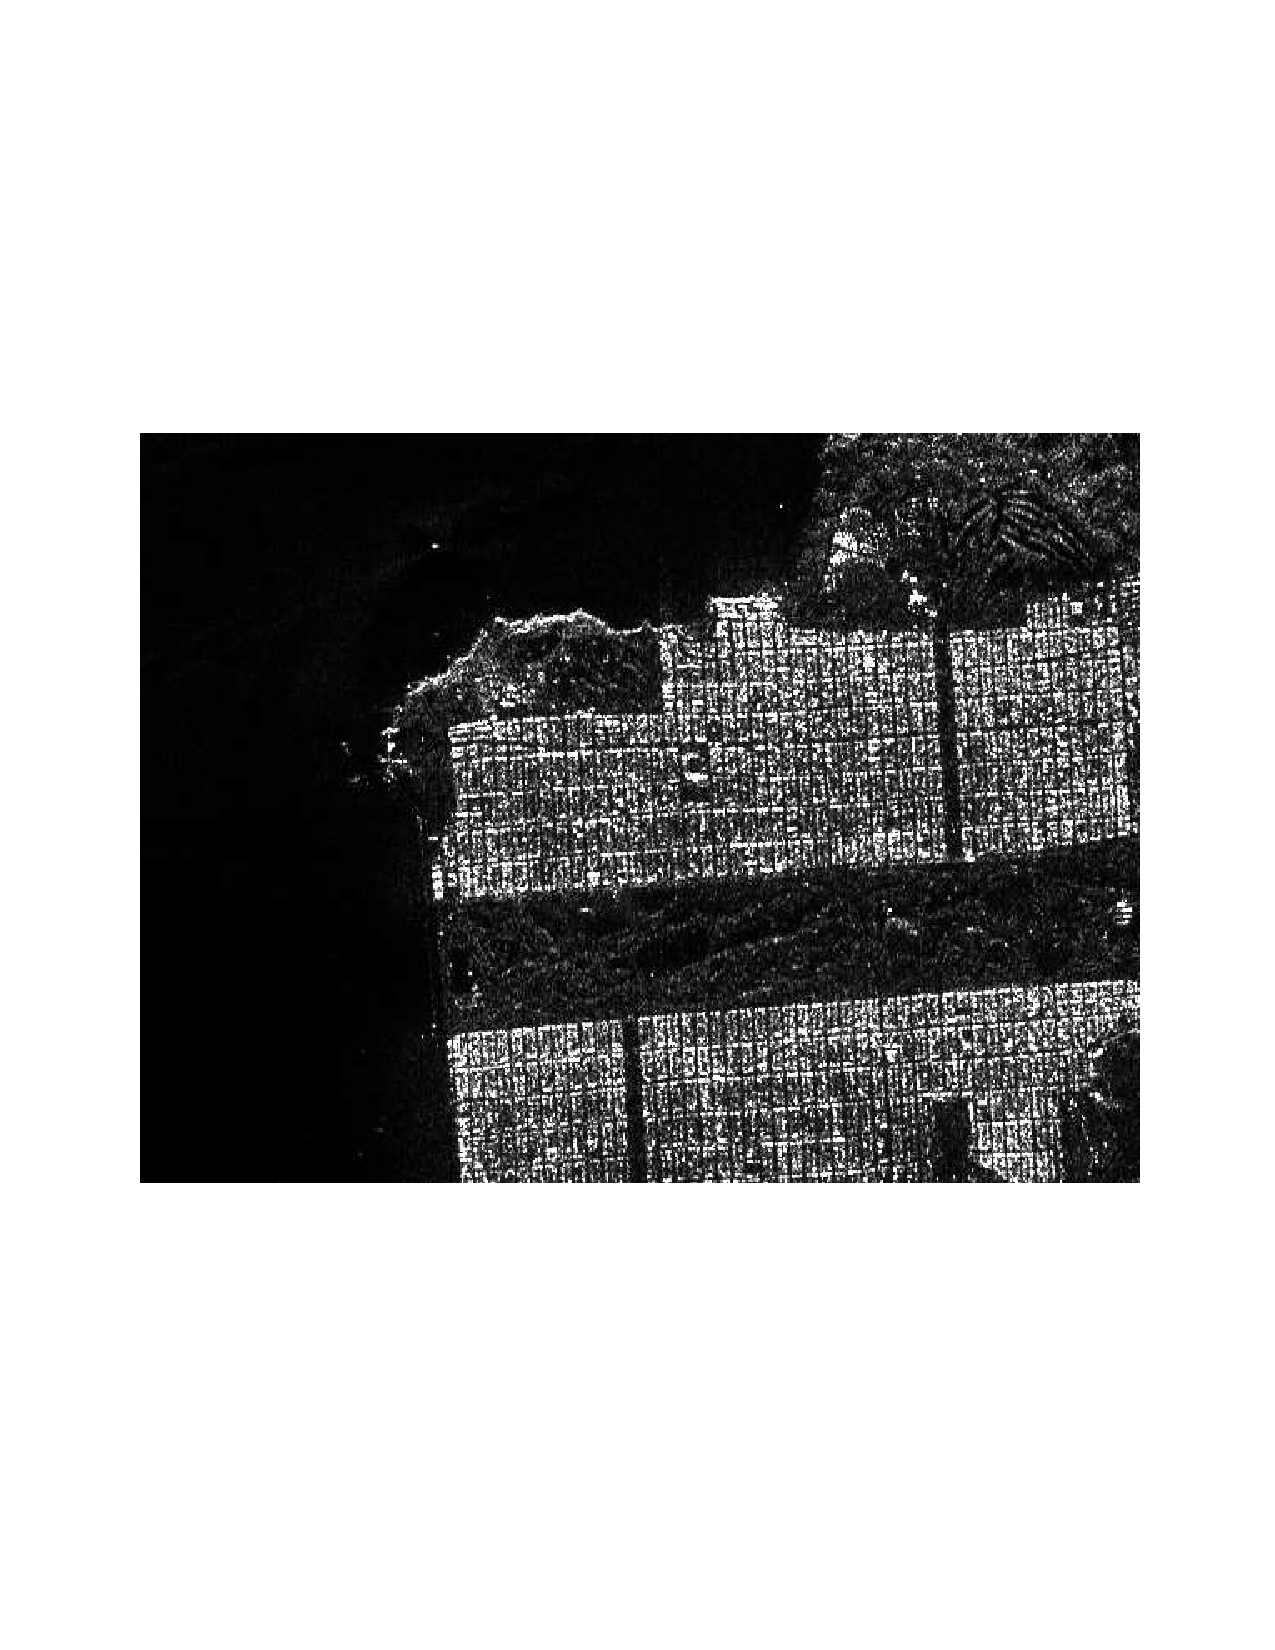
\includegraphics[width=\linewidth]{sf_hh.pdf}
\endminipage
\minipage{0.35\textwidth}
	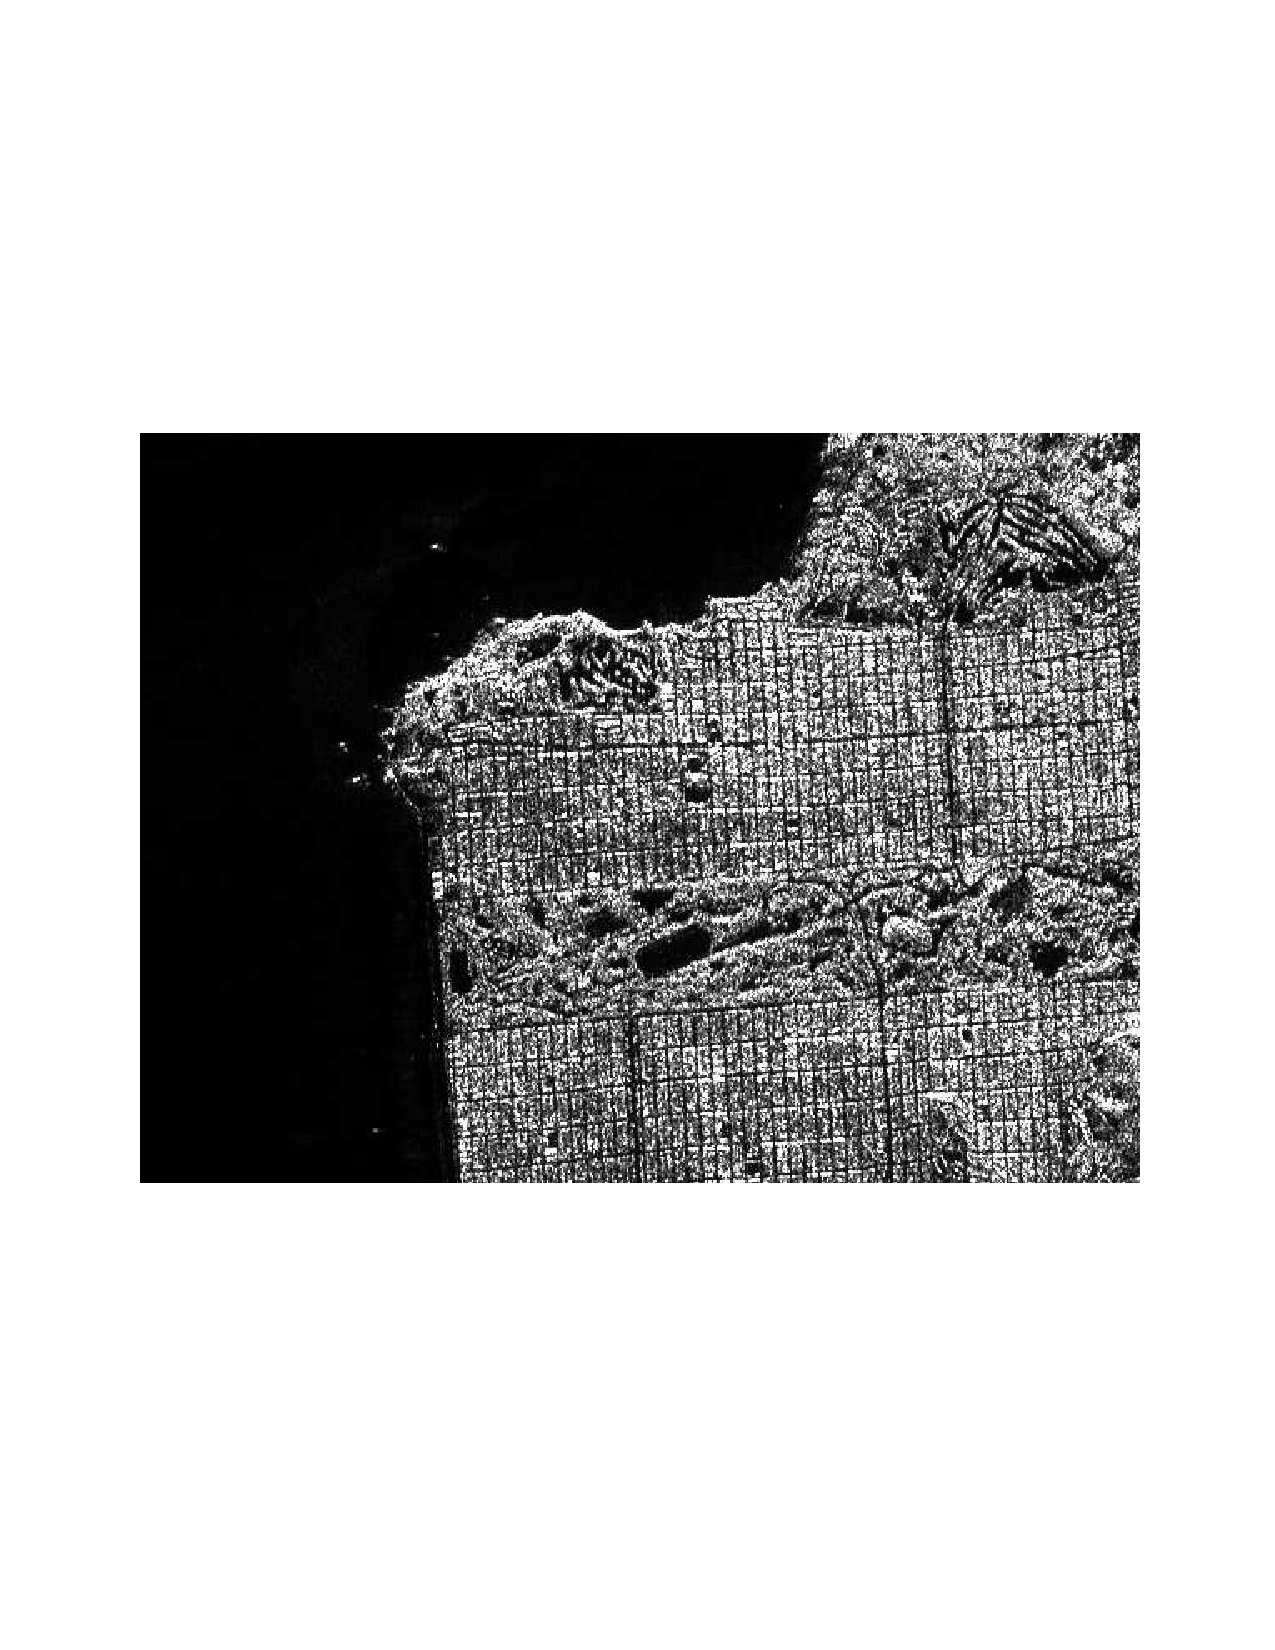
\includegraphics[width=\linewidth]{sf_vh.pdf}
\endminipage
\centering
\minipage{0.35\textwidth}
	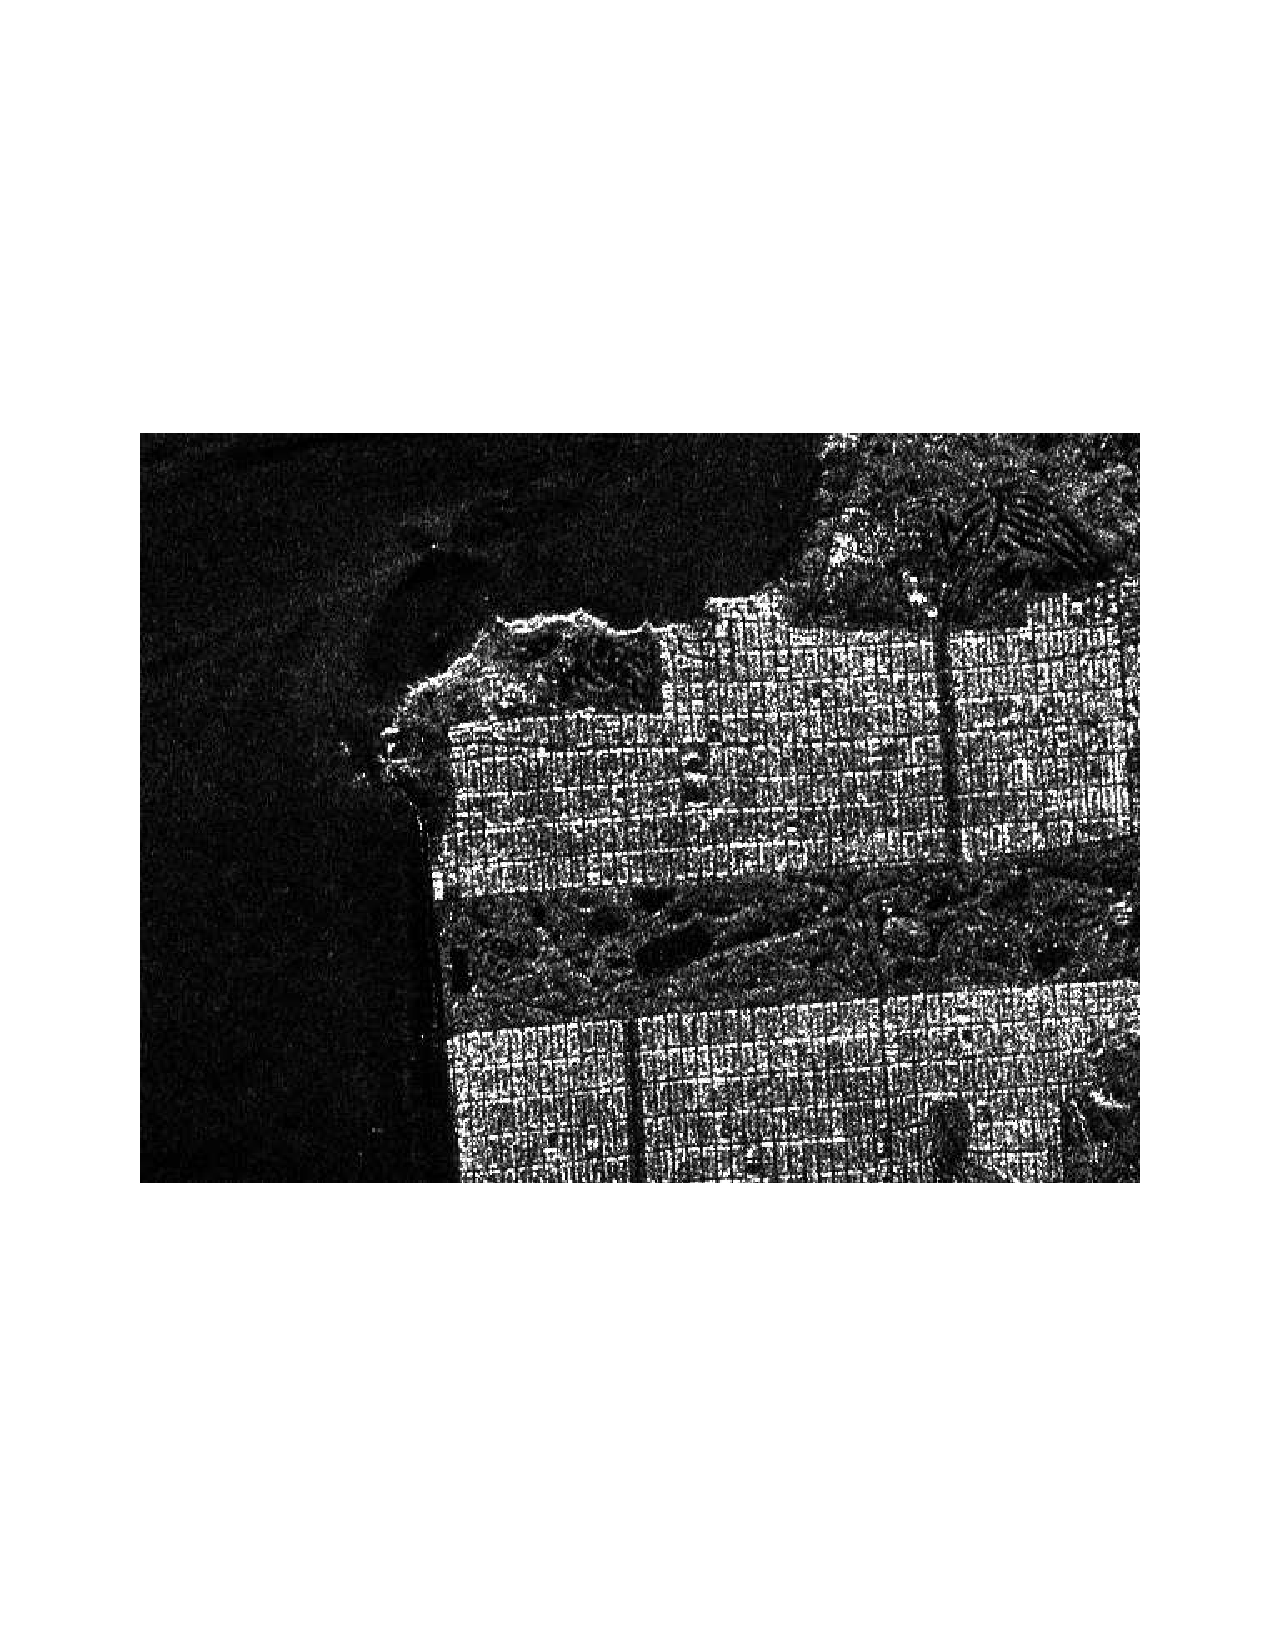
\includegraphics[width=\linewidth]{sf_vv.pdf}
\endminipage
        \vspace{-2.0cm}
	\caption{Imagem PolSAR com polarizações $HH$, $HV$ e $VV$.}\label{cap_acf_sf_hh_hv_vv}
\end{figure}

A visualização usando a decomposição RBG é mostrado na figura (\ref{cap_acf_sf_pauli}), sendo a maneira clássica como é conhecida a imagem da baía de São Franscisco. As figuras (\ref{cap_acf_sf_hh_blue}), (\ref{cap_acf_sf_hv_green}) e (\ref{cap_acf_sf_vv_red}) são respectivamente a decomposição RBG para cada canal $HH$ (azul), $HV$ (verde) e $VV$ (vermelho) das imagens PolSAR. 

\begin{figure}[hbt]
\begin{minipage}[b]{0.450\linewidth}
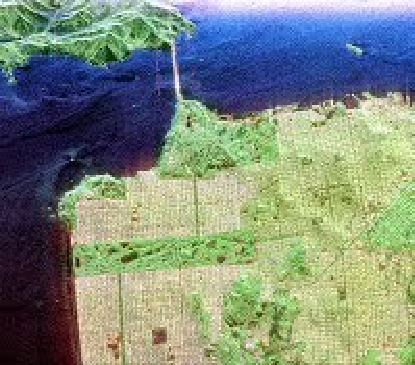
\includegraphics[width=\linewidth]{polsar_teste.pdf}
\caption{Baía de São Francisco.}
\label{cap_acf_sf_pauli}
\end{minipage}\hfill
\begin{minipage}[b]{0.450\linewidth}
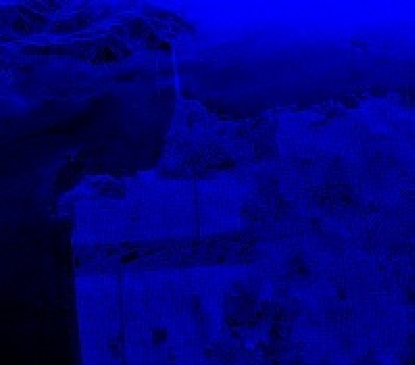
\includegraphics[width=\linewidth]{polsar_blue.pdf}
\caption{Polarização $HH$.}
\label{cap_acf_sf_hh_blue}
\end{minipage}
\end{figure}
%
\begin{figure}[hbt]
\begin{minipage}[b]{0.450\linewidth}
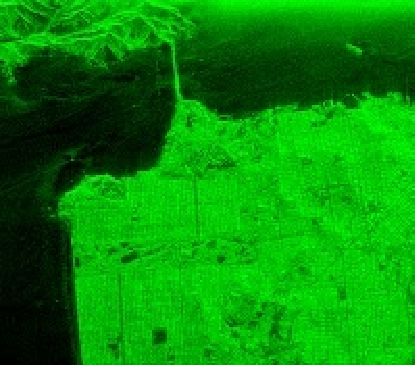
\includegraphics[width=\linewidth]{polsar_green.pdf}
\caption{Polarização $HV$.}
\label{cap_acf_sf_hv_green}
\end{minipage}\hfill
\begin{minipage}[b]{0.450\linewidth}
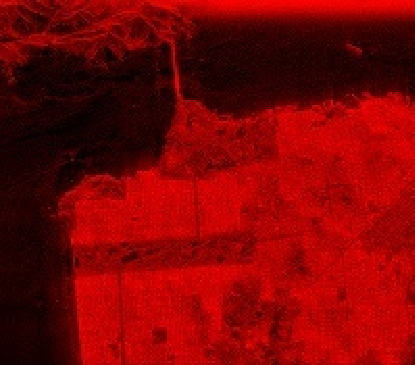
\includegraphics[width=\linewidth]{polsar_red.pdf}
\caption{Polarização $VV$.}
\label{cap_acf_sf_vv_red}
\end{minipage}
\end{figure}

Atualmente, podemos indicar tendências de aplicações de imagens SAR e PolSAR.  Existe interesse em desenvolver um sistema tipo SAR, com comprimentos de ondas óticos que podem ter uma resolução de $10\times 10$ centímetros quadrados, um exemplo é o  sistema Lynx projetado pelo laboratório nacional Sandia, o qual alcança resoluções de $10$ a $30$ centímetros quadrados. Existe ainda o mini-SAR para uso em veículos aéreos não tripulados que focam na evolução da micro-eletrônica para aumentar a eficiência e diminuir o peso. 

As imagens SAR podem ser captadas por satélites orbitando outros planetas como o projeto Magellan SAR orbitando Vênus.  Outra tecnologia usada para a captação  imagens SAR, chamada de interferométrica SAR (InSAR), que usa dois ou mais radares de abertura sintética para obter imagens.   
 
Os sistemas SAR e PolSAR apresentam algumas características inerentes do processo teórico e tecnológico que poderíamos destacar como desvantagens:
\begin{itemize}
\item requer o conhecimento da rota do radar;
\item o sistema SAR é sensível ao movimento do alvo;
\item o processamento para a geração de uma imagem é complexo.
\end{itemize}

Entretanto essas desvantagens nos sistemas SAR e PolSAR não evitam as mesmas de serem largamente empregadas, tornando a área do conhecimento muito ativa, gerando um grande interesse, tanto em nível de aplicação como em pesquisa científica.

